

%To run this example, follow the link
查看本节演示代码：\demonotebook{05}{5.4_DC_QAOA} \ \demonotebookgithub{05}{5.4_DC_QAOA}

\subsubsection{背景}
在量子计算领域，研究人员持续寻求高效且鲁棒的方法来处理复杂问题。绝热量子计算（Adiabatic Quantum Computation, AQC）就是这样一种方法，其中量子系统从初始哈密顿量逐渐演化到编码目标解的最终哈密顿量。根据绝热定理，如果该演化足够缓慢，系统将在整个过程中保持在哈密顿量的基态：
\begin{equation}
    H(t) = (1-\lambda(t))H_{\text{initial}} + \lambda(t)H_{\text{final}},
\end{equation}
其中 \(\lambda(t) \in [0, 1]\)。然而，在实际场景中执行 AQC 会面临外部噪声、器件不完美以及需要长时间演化等挑战。为了克服这些限制并提升绝热演化效率，一个有前景的方案是量子近似优化算法（QAOA）。

QAOA 使用参数化量子线路制备试探态，以近似优化问题的解。通过优化 ansatz 参数，QAOA 寻找使目标函数最小的最优取值，而目标函数编码了问题的能量景观。这种方法能够缩短演化时间，并对噪声和不完美因素具有更强鲁棒性，因此在实际量子计算应用中可作为 AQC 的可行替代方案。

然而，QAOA 的硬件实现仍会受到噪声、退相干以及参数优化复杂性的挑战。为提升其性能和鲁棒性，数字化反绝热量子近似优化算法（Digitized Counterdiabatic Quantum Approximate Optimization Algorithm, DC-QAOA）引入了反绝热（counterdiabatic, CD）项：

\begin{equation}
    H_{\text{DC-QAOA}} = H_{\text{initial}}(\gamma) + H_{\text{final}}(\beta) + H_{\text{CD}}(\alpha),
\end{equation}

该方法结合了绝热量子计算（AQC）与 QAOA 的思想。与 QAOA 相比，它在每层中引入一个额外参数，从而在不牺牲精度的情况下得到更浅的量子线路：
\begin{equation}
    \label{eq:evo operator}
    U(\gamma, \beta) \to U(\gamma, \beta, \alpha), \quad F(\gamma, \beta) \to F(\gamma, \beta, \alpha),
\end{equation}
其中 \(\alpha\)、\(\beta\) 和 \(\gamma\) 表示数字化参数，\(F\) 为代价函数，\(U\) 为演化算符。

CD 项作为哈密顿量中的额外组成部分，基于演化哈密顿量的瞬时本征态和本征能量设计。它能够有效抑制误差并减少所需演化时间，从而提升量子计算的效率和可靠性。

为了推导反绝热项的精确形式，人们已经应用了多种技术，例如 Lewis-Riesenfeld 不变量和无跃迁量子驱动~\cite{PhysRevA.83.062116}。CD 项的实现会根据具体问题和量子系统动力学进行定制，并利用可用控制技术。当难以获得精确 CD 项时，可以采用一种近似 CD 驱动方法，即结合绝热规范势使用嵌套对易子方法~\cite{PhysRevResearch.4.013141}：

\begin{equation}
    A_{\lambda}^{(l)} = i \sum_{k=1}^{l} \alpha_{k}(t) [H_{a}, [H_{a}, \ldots, [H_{a}, \partial_{\lambda} H_{a}]]].
\end{equation}

DC-QAOA 有望用于求解广泛的优化问题，从组合优化到蛋白质折叠~\cite{PhysRevApplied.20.014024} 和金融投资组合优化~\cite{PhysRevResearch.4.043204}。随着量子计算技术持续发展，DC-QAOA 为利用反绝热项和参数空间数字化开拓量子优化新前沿提供了令人期待的途径。

\textbf{目标问题}
\begin{itemize}
    \item[1.] 学习如何寻找问题哈密顿量的基态
    \item[2.] 利用量子线路寻找优化参数
\end{itemize}
\textbf{所需 MindQuantum 功能}
\begin{itemize}
    \item[1.] 基于梯度的优化器
    \item[2.] 批量量子线路模拟器

\end{itemize}

\subsubsection{实现}
作为变分算法的一种成熟变体，该方法需要两个步骤：构建 ansatz 线路和执行优化。现在来看如何将 DC-QAOA 应用于 Ising 模型~\cite{PhysRevResearch.4.013141}。哈密顿量的一般形式由下式给出：

\begin{equation}
    H_{final} = H_{prob} = -J_{ij}\sum_{i=1}^{n-1}\sigma^z_i\sigma^z_{i+1}-h_{i}\sum_{i=1}^{n}{\sigma_i^z} + k_{i}\sum_{i=1}^{n}\sigma_{i}^{x}.
\end{equation}

初态选为 $H_{initial} = \sum_{i}\sigma_{i}^{x}$，它应当驱动不同态之间的跃迁，从而促进对解空间的探索。具体而言，我们选择纵场 Ising 模型（longitudinal field Ising model, LFIM）哈密顿量，其中 $J_{ij}=1,~h_{i}=1,~k_{i}=0$。
\begin{lstlisting}
# 生成作为 H_{mixer} 的 H_{initial}.
# n_qubits 是量子比特数量
def generate_h_mixer(n_qubits:int):
    h_mixer = QubitOperator()
    for i in range(n_qubits):
        h_mixer += QubitOperator(f'X{i}')
    return h_mixer

# 生成作为 H_{prob} 的 H_{final}.
def generate_h_prob(n_qubits:int, J:float, h:float):
    h_prob = QubitOperator()
    for i in range(n_qubits-1):
        h_prob += QubitOperator(f'Z{i} Z{i+1}', -J)
    for i in range(n_qubits):
        h_prob += QubitOperator(f'Z{i}', -h)
    return h_prob
\end{lstlisting}

在本例中，使用绝热规范势的嵌套对易子方法定义一个 CD 算符池~\cite{PhysRevResearch.6.013147}：
$$A = \{\sigma^{y},\sigma^{z}\sigma^{y}, \sigma^{y}\sigma^{z}, \sigma^{x}\sigma^{y}, \sigma^{y}\sigma^{x} \}.$$
这里给出一个 12 量子比特系统，并考虑 CD 项为 $A^{*} = \sum_{i=1}^{n}\sigma_{i}^{y}$。接下来构建 DC-QAOA 的 ansatz 层。
\begin{lstlisting}
def generate_h_cd(n_qubits:int):
    h_cd = QubitOperator()
    for i in range(n_qubits):
        h_cd += QubitOperator(f'Y{i}')
    return h_cd
\end{lstlisting}

\begin{lstlisting}
n_qubits = 12
J, h = 1, 1

h_prob = generate_h_prob(n_qubits, J, h)
h_mixer = generate_h_mixer(n_qubits)
h_cd = generate_h_cd(n_qubits)
\end{lstlisting}

为了制备 $H_{initial}$ 的本征态，我们首先构造 ${\rm prep\_circ}$，随后在其上施加演化算符。
\begin{lstlisting}
# 制备 $H_{mixer}$ 的本征态。
prep_circ = UN(H, n_qubits)
# 选择层数 p。
p = 1

ansatz_template =   u_p + u_m  + u_cd

ansatz = Circuit() + prep_circ

for i in range(p):
    ansatz += add_suffix(ansatz_template, str(i)) + BarrierGate()
\end{lstlisting}

只要设置好了 ansatz 线路，就可以改变层数或经典优化器类型，以寻找最优参数集合。我们定义代价函数为
\begin{equation}
    F(\alpha,~\beta,~\gamma) = \left<\psi_0\right|U^{\dagger}\ H_{prob} U\left|\psi_0\right>,
\end{equation}
其中 $U = \Pi_{i=0}^p U_{cd}(\alpha_i)U_m(\beta_i)U_p(\gamma_i)$，这正是式~\ref{eq:evo operator} 中的演化算符。
\begin{lstlisting}
def train(ham, ansatze, iteration):

    # 构建量子线路

    circ = ansatze
    sim = Simulator('mqvector', ansatze.n_qubits)

    grad_ops = sim.get_expectation_with_grad(ham, circ)
    net = MQAnsatzOnlyLayer(grad_ops)
    opti = nn.Adagrad(net.trainable_params(), learning_rate=0.05)
    train_net = nn.TrainOneStepCell(net, opti)

    result = []
    for i in range(iteration):
        train_net()
        result.append(np.array(train_net()[0]))
    pr = dict(zip(ansatze.params_name, net.weight.asnumpy()))

    return result
\end{lstlisting}

在本教程中，我们使用 Adam 优化器~\cite{PhysRevResearch.6.013147} 优化梯度，它能够给出足够好的结果。绘制平均能量图后可得到图~\ref{fig:dc}。其中，绿色虚线是 $H_{prob}$ 的精确本征值，蓝色实线是一层 DC-QAOA 在优化过程中的平均值，橙色实线是一层 QAOA 的结果。可以看到，DC-QAOA 在 20 步内已经收敛到精确值，而 QAOA 则陷入局部最小值。从估计基态的能力来看，DC-QAOA 相比 QAOA 具有优势。
\begin{figure}
    \centering
    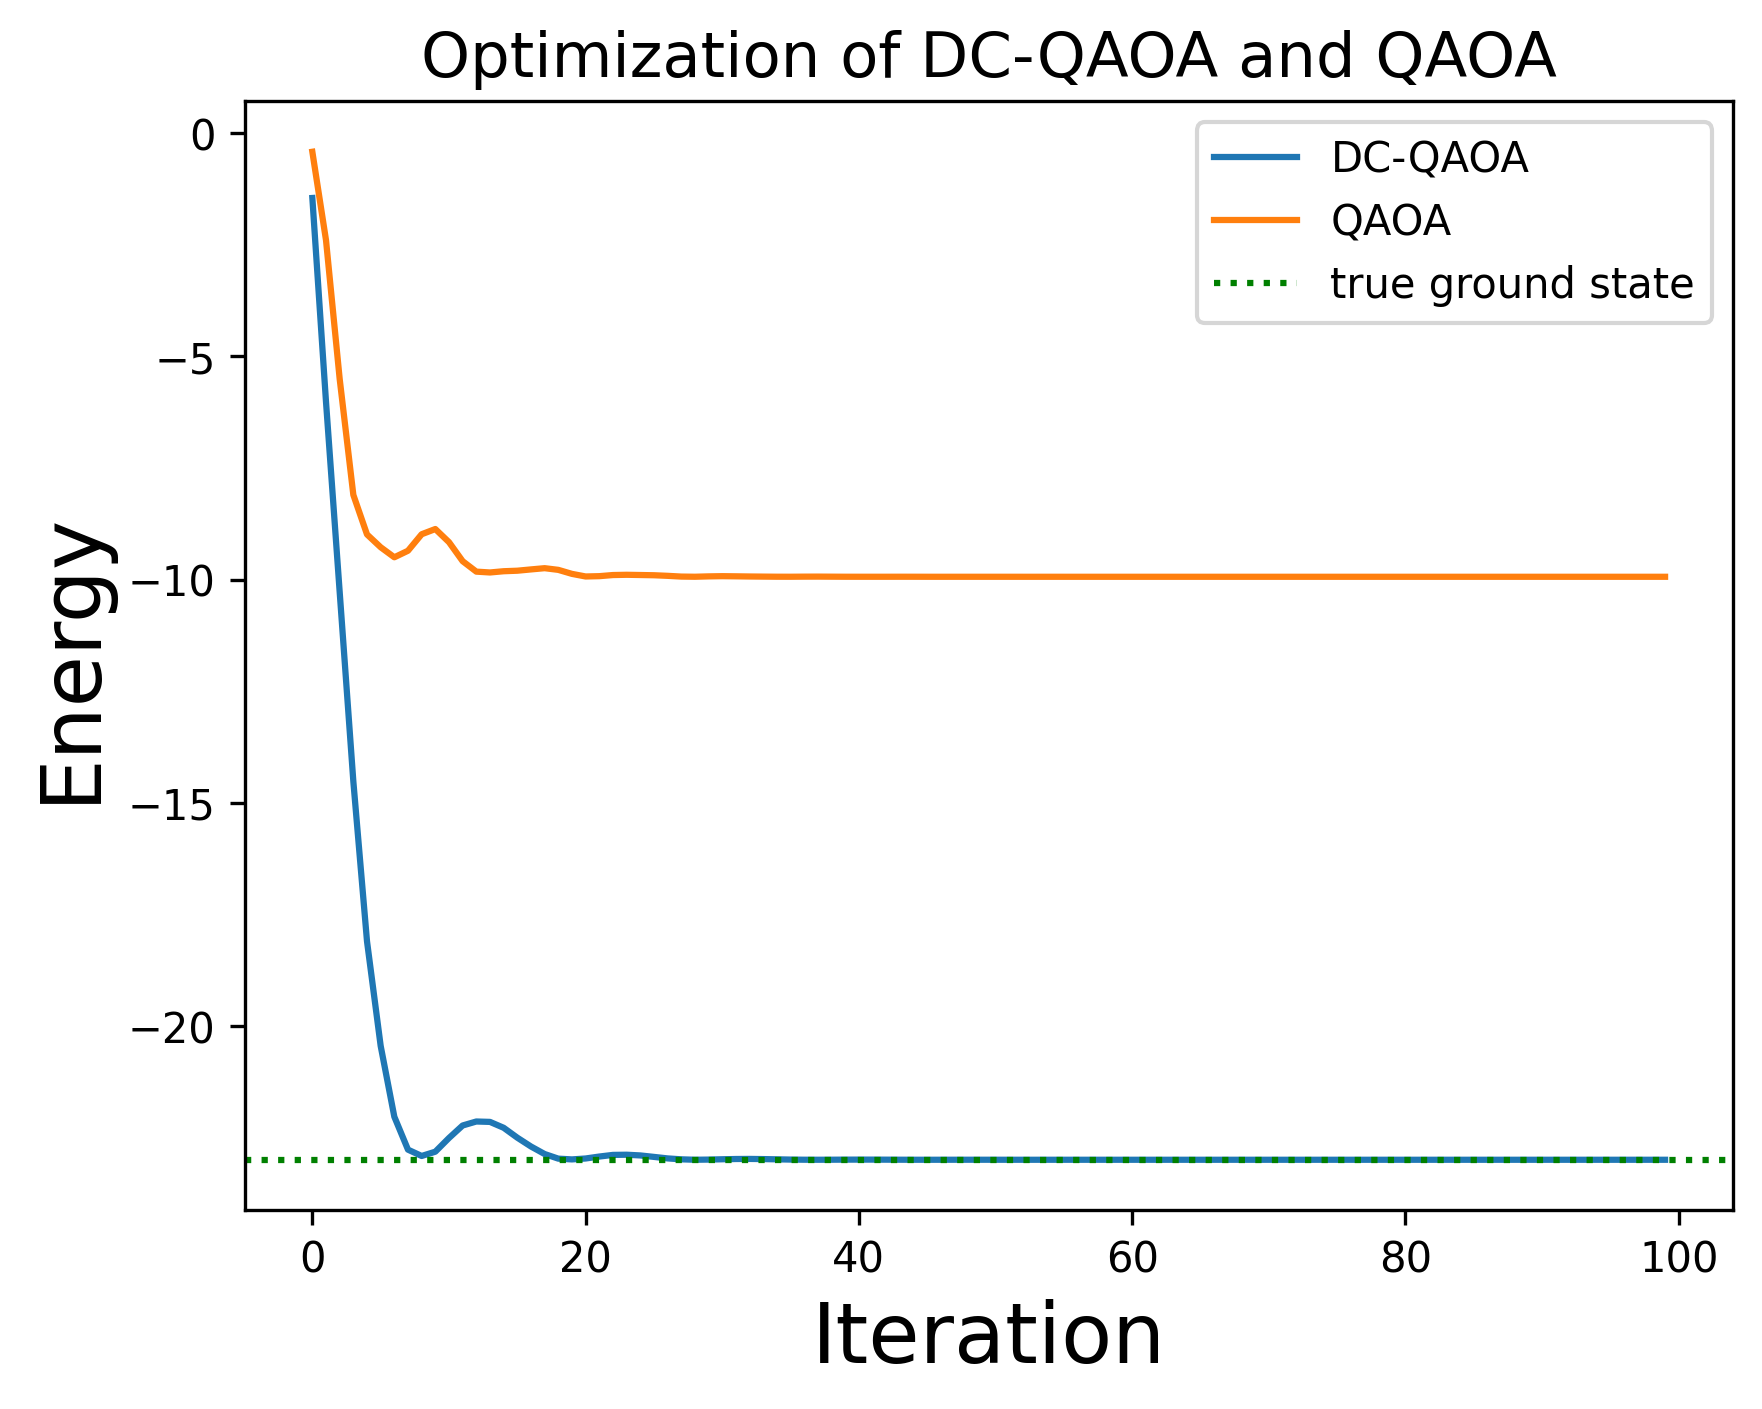
\includegraphics[width = 1 \linewidth]{5.4.1_figure/DC-QAOA.png}
    \caption{能量随迭代次数的变化。}
    \label{fig:dc}
\end{figure}
